% !TEX root = scientific-computing.tex

% this needs to be at the top of each file with the \plot command and the word in the [] is the session for pythontex. 
\begin{jlcode}[numint]
using Plots, PGFPlotsX
pgfplotsx()
\end{jlcode}

\chapter{Numerical Integration} \label{ch:num-int}

Numerical integration is a very important component of scientific computation.  In tradition calculus classes, the integrals presented were ones that had antidervatives that could be found relatively easily.  However, this is generally not true.  For example, if trying to determine

\begin{align*}
\int_0^{2} e^{-x^2} \, dx 
\end{align*}
%
the function $f(x)=e^{-x^2}$ does not have an antidervative in terms of standard functions.  This however it a very important antidervative in that it is related to the normal probability distribution.  Because of its importance, we define
\begin{align*}
\text{erf}(x) & = \frac{2}{\sqrt{\pi}} \int_0^x e^{-t^2} \, dt 
\end{align*}
as the \href{https://en.wikipedia.org/wiki/Error_function}{error function} it is important to calculate values for it for any value of $x$.  

\section{Trapezoid Rule}

%% simple trap rule code:
\begin{jlcode}[numint]
function trapRule(f::Function, a::Real, b::Real, n::Integer)
  n > 0 || throw(ArgumentError("The number of trapezoids, n, must positive."))
  a < b || throw(ArgumentError("The left endpoint must be less than the right endpoint."))
  local h = (b-a)/n
  local xpts = LinRange(a,b,n+1)
  (h/2)*(f(a)+f(b) + 2*sum(f,xpts[2:end-1]))
end
\end{jlcode}



Instead of approximating the area with rectangles, we can use trapezoids to do this.  A plot of the approximate integral of $e^{-x^2}$ on the interval $[0,2]$ is given by

\begin{center}
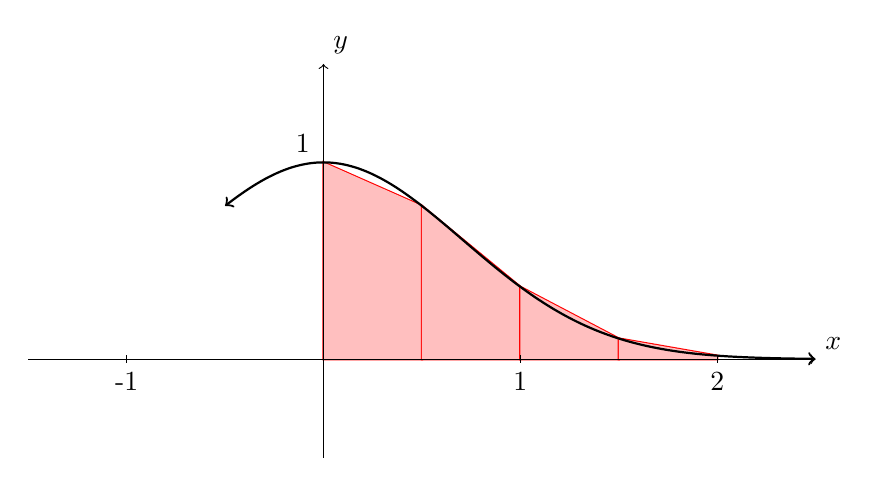
\begin{tikzpicture}[scale=2.5]

\draw[red,thick] (0,1) -- (0.5,{exp(-0.5*0.5)}) -- (0.5,0) -- (0,0) -- cycle;
\fill[pink] (0,1) -- (0.5,{exp(-0.5*0.5)}) -- (0.5,0) -- (0,0) -- cycle;
\draw[red,thick] (0.5,0) -- (0.5,{exp(-0.5*0.5)}) -- (1,{exp(-1)}) -- (1,0) -- cycle;
\fill[pink] (0.5,0) -- (0.5,{exp(-0.5*0.5)}) -- (1,{exp(-1)}) -- (1,0) -- cycle;
\draw[red,thick] (1,0) -- (1,{exp(-1)}) -- (1.5,{exp(-1.5*1.5)}) -- (1.5,0) -- cycle;
\fill[pink] (1,0) -- (1,{exp(-1)}) -- (1.5,{exp(-1.5*1.5)}) -- (1.5,0) -- cycle;
\draw[red,thick] (1.5,0) -- (1.5,{exp(-1.5*1.5)}) -- (2,{exp(-4)}) -- (2,0) -- cycle;
\fill[pink] (1.5,0) -- (1.5,{exp(-1.5*1.5)}) -- (2,{exp(-4)}) -- (2,0) -- cycle;
\draw[<->,thick] plot[samples=150, domain=-0.5:2.5] (\x,{exp(-1*\x*\x)});

\draw[->] (-1.5,0) -- (2.5,0) node [above right] {$x$}; 
\foreach \x in {-1,1,2} \draw (\x,0.02) -- (\x,-0.02) node [below] {\x}; 
\draw[->] (0,-0.5) -- (0,1.5) node [above right] {$y$}; 
\foreach \y in {1} \draw (0.02,\y) -- (-0.02,\y) node [above left] {\y};


\end{tikzpicture}
\end{center}
where 4 trapezoids have been used.  The area of the a trapezoid like: 
\begin{center}
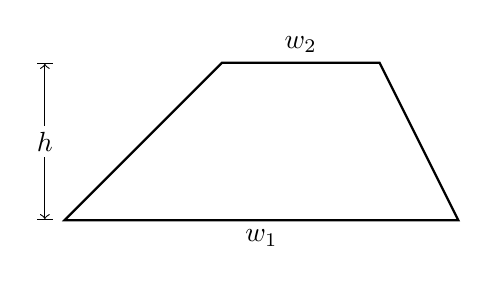
\begin{tikzpicture}
\draw[thick] (0,0) -- (5,0) -- (4,2) -- (2,2) -- cycle;
\draw (2.5,0) node [below] {$w_1$};
\draw (3,2) node [above] {$w_2$};
\draw[|<-] (-0.25,0) -- (-0.25,0.8);
\draw (-0.25,1) node {$h$};
\draw[->|] (-0.25,1.2) -- (-0.25,2); 
\end{tikzpicture}
\end{center}
%
is
\begin{align*}
A & = \frac{1}{2} h (w_1+w_2)
\end{align*}

In the trapezoids in the function plot above, the trapezoid are oriented sideways to this one, so the value of $h$ is the horizontal distance or 0.5 for each one and the $w_1$ and $w_2$ are the function values, so the area of the four trapezoids above are:
\begin{align*}
A & = \frac{0.5}{2} \bigl(e^0 + e^{-0.5^2} \bigr) + \frac{0.5}{2} \bigl(e^{-0.5^2} + e^{-1} \bigr) + 
\frac{0.5}{2} \bigl(e^{-1} + e^{-1.5^2} \bigr) + \frac{0.5}{2} \bigl(e^{-1.5^2}+ e^{-2^2} \bigr) \\
& \approx \jl[numint]{trapRule(x->exp(-x^2),0,2,4)}
\end{align*}

The basic part of the trapezoid method is to use the area of a trapezoid on an interval with width $h$.  The area of one of the trapezoids is
%
\begin{align*}
A_i = \frac{h}{2}(f(x_i)+f(x_{i+1}))
\end{align*}
%
and then a full approximation will be the sum of these:
\begin{align}
A& ={\sum_{i=1}^{n-1}} \frac{h}{2}(f(x_i)+f(x_{i+1})) \notag \\
 & =\frac{h}{2}\left(f(x_0)+f(x_1)+f(x_1)+f(x_2)+ \cdots + f(x_{n-1})+f(x_n)\right) \label{eq:trap:rule:1} \\
 & =\frac{h}{2}\left( f(x_0) + \biggl(2\sum_{i=1}^{n-1} f(x_i) \biggr) + f(x_n)\right) \label{eq:trap:rule}
 \end{align}

Let's take a look at doing this in julia.  To calculate the value we need a few things: 1) a function, 2) the interval we're doing the approximation on and 3) the number of trapezoids or subintervals.  We presented the following in Chapter \ref{ch:adv-functions} as 
\begin{jlblock}[numint]
function trapRule(f::Function, a::Real, b::Real; num=10)
  local h = (b-a)/num
  0.5*h*sum(map(f,collect(a:dx:b-dx))+map(f,collect(a+dx:dx:b)))
end
\end{jlblock}

\begin{enumerate}
\item The parameter $h$ is $(b-a)/n$.
\item Line (\ref{eq:trap:rule:1}) can be written as the map of two arrays. And then summed. 
\end{enumerate}

This is short and (maybe) sweet, but note that there are two separate arrays created.  We have learned throughout this text, that the creation of arrays is often the most expensive part of a calculation.  So instead, we will do the following: 

\begin{jlblock}[numint]
function trapRule(f::Function, a::Real, b::Real; num = 10)
  num > 0 || throw(ArgumentError("The number of trapezoids, num, must positive."))
  a < b || throw(ArgumentError("The left endpoint must be less than the right endpoint."))
  local h = (b-a)/num
  (h/2)*(f(a)+f(b)+2*sum(f,LinRange(a+h,b-h,num-1)))
end
\end{jlblock}

Although this looks to be nearly the same, we haven't created arrays.  The \texttt{LinRange} function creates a range, but julia is savvy enough to not create the array to sum over it. See the exercise below.

Let's first redo the example above: 
\begin{jlblock}[numint]
trapRule(x->exp(-x^2),0,2;num=4)
\end{jlblock}
which returns \jlc[numint]{print(trapRule(x->exp(-x^2),0,2;num=4))} \printpythontex[verb].

\subsection{Exercise}
\begin{itemize}
\item Find $\int_0^{1} \sin(x^2)\,dx$ using the trapezoid method for $4, 10$ and $20$ points.  
\item Use the \texttt{BenchmarkTools} and the \texttt{@btime} macro to compare the time of the trapezoid rule using the two functions shown here. Try integrating $\sin(x^2)$ on $[0,1]$ for $N=10,000$ subintervals. 
\end{itemize}


\section{Simpson's Rule}

The trapezoid rule uses straight lines to approximate the function and then integrates the line (or finds the area of the trapezoid).  To find a better approximation if we use a quadratic function (parabola) to estimate the function.  If we do this, then integrate the resulting parabola, this is called Simpson's Rule.  There are numerous places to find the derivation of this, but the result is 

\begin{align*}
I & = \frac{h}{3} \bigl( f(x_0) + 4 f(x_1) + 2 f(x_2) + 4 f(x_3) + 2 f(x_4) + \cdots + 2 f(x_{n-1}) + f(x_n) \bigr) \\
& = \frac{h}{3} \left(f(x_0)+ f(x_{2n}) + 4 \sum_{k=1}^{n} f(x_{2k-1}) + 2\sum_{k=1}^{n+1} x_{2k} \right) 
\end{align*}
where $h=(b-a)/n$, $x_k = a + kh$ and it is important that $n$ is an even number. 

Similar to the trapezoid rule, we can write Simpson's rule in julia as 

\begin{jlblock}[numint]
function simpsonsRule(f::Function, a::Real, b::Real, n::Integer) 
  n > 0 || throw(ArgumentError("The number of subintervals, n, must be positive."))
  n % 2 == 0 || throw(ArgumentError("The number of subintervals, n, must be even."))
  a < b || throw(ArgumentError("The left endpoint must be less than the right endpoint."))
  local h = (b-a)/n
  xpts = LinRange(a,b,n+1)
  (h/3)*(f(a)+f(b) + 4*sum(f,xpts[2:2:end-1]) + 2*sum(f,xpts[3:2:end-2]))
end
\end{jlblock}

Applying Simpson's Rule to $\int_0^3 x^2 \, dx$ as \jlb[numint]{simpsonsRule(x->x^2,0,3,10)} results in \jlc[numint]{print(simpsonsRule(x->x^2,0,3,10))} \printpythontex[verb].  It's interesting to note that this reports the exact value.  In fact, Simpson's rule will numerically integrate any cubic (and lines and quadratics) exactly.  

If we return to trying to find $\int_0^2 e^{-x^2} \, dx$ and use Simpson's Rule, then 
\begin{jlblock}[numint]
simpsonsRule(x->exp(-x^2),0,2,10)
\end{jlblock}
returns \jlc[numint]{print(simpsonsRule(x->exp(-x^2),0,2,10))} \printpythontex, which is within 5 digits of the true answer.  

\subsection{Plotting the Error Function}

We can use numerical integration to evaluate the error function at any value, so let's go ahead and plot it. 

First, let's make a function that defines the error function. 

\begin{jlblock}[numint]
function erf(x::Real)
  local area = simpsonsRule(t->exp(-t^2),0,abs(x),100)
  x > 0 ? area : -1*area
end
\end{jlblock}
where we have used the symmetry of the error function to evaluate it if \verb!x! is positive or negative.  If we don't check for this, we will get an error because \verb!simpsonsRule! has a check that the interval needs to be put in as $a<b$.  


Now, we can plot it with:
\begin{jlblock}[numint]
plot(x->erf(x), -3, 3, label=false, title="Plot of the error function")
\end{jlblock}
which results in 
\begin{center}
\plot{plots/numerical-integration/erf.tex}{numint}
\end{center}


\section{Using the \texttt{NumericalIntegration} package} 

This package does some basic integration using both Trapezoid and Simpson's rule discussed above. 
\begin{jlblock}
using NumericalIntegration
x = LinRange(0,2,101)
y = map(x->exp(-x^2),x) ## compute an array of y based on each x
v = integrate(x,y)
\end{jlblock}
and the result is \jlc{print(v)} \printpythontex


{\color{red} not impressed with this package. Maybe I shouldn't include this.  If we decide to, need to expand and show some of the details.} 
